\documentclass[runningheads]{llncs}
%
\usepackage{graphicx}
\usepackage[nottoc]{tocbibind}
\usepackage[
backend=biber,
style=chem-biochem,
]{biblatex}
\usepackage{hyperref} 
\addbibresource{docs/pentacode.bib} 

\begin{document}

%
\title{REMAILLAGE ET SIMPLIFICATION DE
MAILLAGES QUADRANGULAIRES 3D}
%
%\titlerunning{Abbreviated paper title}
% If the paper title is too long for the running head, you can set
% an abbreviated paper title here
%
%\author{Lowin Kossel\inst{1} \and
%Clement Lefranc\inst{1} \and
%Marco Flores\inst{1} \and
%Alexandre Bordes\inst{1}}

\authorrunning{Pentacode}

\institute{Université Toulouse 3 - Paul Sabatier}
%
\maketitle              % typeset the header of the contribution
%

\begin{abstract}
Dans cet état de l'art nous allons mettre en perspective les différentes méthodes pour passer d'un maillage triangulaire à maillage quadrangulaire en les comparants sur différents critères comme leurs robustesses, leur rapidité, leur efficacité et enfin leur adaptabilité. Nous passerons en revue les techniques de simplification de maillage quadrangulaire avec leur avantage et inconvénient.

\keywords{Remaillage quadrangulaire  \and Simplification de maillage quadrangulaire}
\end{abstract}

\section{Introduction}
\subsection{Motivation et Context}
Dans de nombreux domaines où l'on a besoin de représenter informatiquement des objets en 3D( infographie, architecture, mécanique, etc… ), la plupart des applications utilisent une représentation via un maillage polynomial. Cette représentation est basée sur l’assemblage de plusieurs polygones pour créer le maillage, les plus utilisés sont les triangles et les quads. Les maillages quadrangulaires (maillage composé uniquement de quads), trouve plusieurs avantages comparées aux maillages triangulaires, cela est dû au fait que les quads ont naturellement la capacité de détecter les principaux champs directionnels de courbure et à partager un domaine commun avec les solutions de paramétrage de surface.  On le retrouve ainsi majoritaire dans le domaine de l'animation, pour la modélisation de "high-order" surface et pour réaliser du texturing et de la compression. Cette démocratisation de l’utilisation des quads pousse naturellement à développer de nouvelles méthodes pour réaliser de la simplification de maillage quadrangulaire. L'attrait pour la simplification de mesh est dû au fait qu’elle est un élément de base et indispensable du traitement géométrique qui est intrinsèquement lié au rendu, à la compression du maillage, à la reconstruction de forme, etc….


\subsection{Base thérorique et Définition}
\begin{figure}
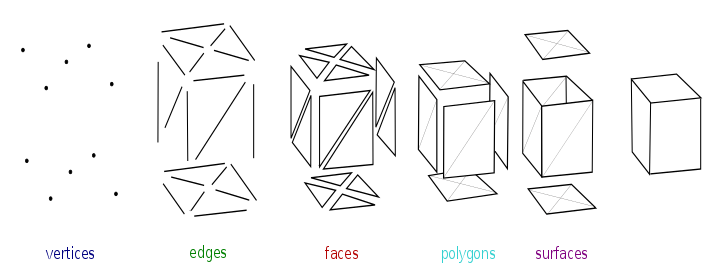
\includegraphics[width=\textwidth]{img/geom-def.png}
\caption{Composantes principales d'un maillage polynomiale} \label{fig1}
\end{figure}

Un maillage est définie par un “assemblage de polygone”, un polygone est composé d’une face qui est elle-même composée par des edges composés de vertices.
\begin{itemize}
  \item \textbf{Vertices :} un point à une coordonées donnée dans l’espace
  \item \textbf{Edges :} un segment qui relie deux vertices
  \item \textbf{Faces :} un cycle de plusieurs edges
\end{itemize}
Une mesh constituée uniquement de triangle est appelée mesh triangulaire, alors qu’une mesh constitué uniquement de quads est appelée mesh quadrangulaire. Ici les solutions explorées considèrent qu’on a un maillage conforme en entrée c'est-à-dire que chacune des faces ne partagent qu’un edge entre elles ou un seul vertice.
Chaque edges peut être classé en fonction de ses caractéristique on dit qu’un edge est :
\begin{itemize}
  \item \textbf{Boundary} : si il est adjacent à exactement une face
  \item \textbf{Régulier} : si il est adjacent à exactement deux faces
  \item  \textbf{Singulière}: si il est adjacent à plus de deux faces
\end{itemize}

Les maillages quadrangulaire peuvent être réparties en plusieur type en fonction de leur degré de régularité :
\begin{itemize}
  \item \textbf{Régulier} : Correspond à un pavage de quads régulier
  \item \textbf{Semi-régulier} : Assemblage de sous-maillage (path) de quads 2d régulier
  \item \textbf{Valence Semi-régulier} :Assemblage de sous-maillage (path) 2d de quads régulier qui ou chaque vertices à 4 valences
  \item  \textbf{Unstructured}: Un grand nombre de vertices ne sont pas régulier, souvent obtenu en coupant les triangles d’un maillage triangulaire en trois quads.

\end{itemize}

Dans la simplification des maillages quadrangulaire, les techniques s'appuient sur plusieurs opérations locales sur le maillage. L'effondrement des bords, consiste à faire bouger un vertice le long d’une edge pour rejoindre un autre vertice et remplacer l’un par l’autre, ceci permet donc aussi à la mesh d'être moins lourde en mémoire car elle contiendra moins de points. Et une autre opération très utilisée est l'effondrement des diagonales, qui permet de supprimer un quad en rassemblant les quads qui l’entour.
Rotation des eges et des vertex sont d'autres opérations utilisées dans la simplification de mesh. Elles permettent respectivement de faire tourner un edge entre deux faces, et de faire changer les vertex constituant un quad, entre plusieurs faces.

\subsection{Définition détaillée du problème}
 Le remaillage de maillage triangulaire en quadratique actuelle à plusieurs problèmes, il n’existe pas encore d’algorithme qui permette de réaliser une remaillage de façon rapide avec une forte robustesse. Dans le cas des algorithmes qui permettent d’aller plus vite, on retrouvera un nombre de singularités plus grande. Il faut donc réussir le bon compromis 

\section{Travail réalisé dans le domaine}
\subsection{Organisation structuré de la littérature existante}
On distingue deux approches pour obtenir un maillage quadrangulaire d’une surface: quad conversion et quad remeshing. Vu que dans la majorité des applications les surfaces sont surtout définie avec des maillages triangulaires, Quad conversion essaye de résoudre le problème de convertir un maillage triangulaire a un maillage quadrangulaire. Ceci-dit, quad remeshing implique plutôt un rééchantillonnage de la surface. Une des méthodes les plus populaires consiste à partitionner la surface originelle dans des patches de façon à échantillonner les quads dans ce domaine.Une méthode consiste à réaliser une paramétrisation globale de la surface. Cela permet de créer un domaine dans lequel la création des quads est trivial. De plus, on a des méthodes basées sur la création des champs alignés dans lesquels, en traçant les lignes du champ, on peut remailler la surface en quads. Enfin on a des méthodes qui ne contraignent pas à générer des quads rectangulaires mais permettent la définition d'éléments rectangulaires, c’est-a-dire on permet l'anisotropie.

\subsection{Bref description de chaque domaine et les travails plus représentatives}
\subsubsection{Conversion Tri-to-quad:}

Cette classe de méthodes combine une séquence d'opérations locales sur les connectivités pour convertir un maillage triangulaire en maillage quadrangulaire. Le mécanisme principal consiste à fusionner deux triangles d’origine en quadrilatère, donc la conversion d’un maillage triangulaire en maillage quadrangulaire est basé sur l’appariement de triangles adjacents d’origine. Cette classe de méthode peut seulement espérer la production de maillages quadrangulaires non structurés, non réguliers. Pour obtenir un maillage quadrangulaire pure avec cette méthode, le maillage d’origine doit avoir un nombre pair de triangles. Cela est toujours le cas pour des maillages fermés, sinon cela peut être trivialement forcé en séparant une bordure de triangle en deux. Plusieurs de ces méthodes ont été présentées, souvent en tant que résultats secondaires dans des articles portant sur d’autres parties de domaines connexes.
La technique de [Lai et Al. 2008]\cite{lai_incremental_2008} consiste à appliquer un schéma de relaxation de façon itérative pour aligner les bords du maillage sur les directions principales de la surface, puis de supprimer les diagonales non alignées du maillage triangulaire. Le point crucial de l’algorithme est le mouvement incrémental des sommets pour aider l’alignement sur la direction principale. L’algorithme ne permet de gérer la résolution du maillage de sortie, qui reste corrélé avec le nombre de vertex de du maillage initial. 

\subsubsection{Définition des patches sur la surface}
{Dans cette classe de méthode, le but est de transformer les maillages
d'entrée en un ensemble de patch polygonaux qui à leurs tours seront
transformés en surfaces quadrangulaire. Souvent il faut appliquer
certains prétraitements sur les maillages en entrée afin de détecter les
patchs et d'assurer qu'ils répondent le mieux aux besoins. Ensuite les
patches seront également quadrangulaire en utilisant différentes
méthodes en fonction du besoin. Un patch polygonal est un ensemble de
vertices. Le contour du patch peut être subdivisé en un certain nombre
de segments. Les segments qui séparent 2 vertices représentent les côtés
du patch.}

Certaines méthodes [Campen et Al. 2012]\cite{campen_dual_2012}, [Huang et Al. 2008]\cite{huang_spectral_2008} s’appuient sur le fait de directement construire des patches quadrilatérales afin de rendre la quadrangulation de ces patches plus facile. [Huang et Al. 2008]permet même de paramétriser le processus pour donner certaines propriétés souhaitées aux patches.
D’autres méthodes comme [Pietroni et Al. 2021]\cite{pietroni_reliable_2021} construisent des patches qui ne sont pas nécessairement quadrilatérales. Ces patches seront ensuite quadrangulés via des méthodes de quadrangulation générales [Tarini, Marco 2021]\cite{tarini_closed-form_2021}, [Takayama et Al. 2014]\cite{takayama_pattern-based_2014}. Ces méthodes de quadrangulation de patches s’appliquent sur une grande majorité de patches, des patches de 2 à 6 côtés pour [Takayama et Al. 2014]\cite{takayama_pattern-based_2014} et des patches avec n côtés (avec n supérieur ou égal à 2) pour [Tarini, Marco 2021]\cite{tarini_closed-form_2021}.

\begin{figure}
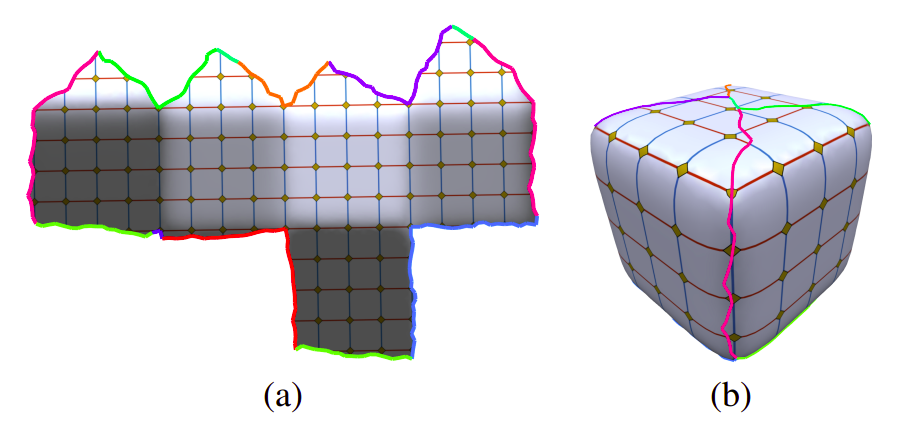
\includegraphics[width=\textwidth]{img/clement_enerve.png}
\caption{L’approche basée sur la paramétrisation coupe et aplatie la surface sur le domaine (a) telle qu’une tessellation quadratique triviale du domaine colle à un maillage quadrangulaire valide sur la surface (b).} \label{fig1}
\end{figure}

\subsubsection{Méthodes basés sur la paramétrisation:}Une formulation du problème global de paramétrisation et les contraintes nécessaires à la quadrangulation partagées par les méthodes conformes / harmoniques et guidées par le champ partagent une même vue de la paramétrisation globale.
On suppose que la surface est coupée par un ensemble de courbures sur un disque topologique ou plusieurs disques. Le principe des méthodes basées sur la paramétrisation est la construction d’un mapping de la surface en 3D dans un domaine en 2D tel que la quadrangulation dans le domaine devient trivial. La plupart du temps le domaine est tesselé par des carreaux réguliers comme le maillage de quad canonique formé par la grille cartésienne des isolignes entières.
Un exemple est montré sur la Figure 2 où un cube lisse est paramétré (a) tel que la grille des isolignes entières est collée à un maillage quadrangulaire sur la surface (b). La partie difficile dans ce cadre est le design de conditions consistantes qui assure un assemblage correct des isolignes le long du graphe coupé qui est essentiels pour les disques non topologiques.

La méthode proposée par [Li et Al. 2011]\cite{li_meshless_2011} permet de générer le maillage quadrangulaire à partir d’un nuage de points. L’algorithme détermine les directions principales, puis applique un K-PPV pour obtenir le champ de direction lisse. La paramétrisation globale est calculée et le gradient est aligné avec le champ de direction. C’est donc à partir de cette paramétrisation qu’on échantillonne les quads de la surface.


\subsubsection{Méthodes guidées par les champs:}
Cette classe de méthodes est caractérisée par un contrôle explicite des propriétés locales des éléments quadrangulaire dans le maillage par les moyennes des champs de guidage. Typiquement, les propriétés locales les plus intéressantes sont l’orientation et la taille des éléments quadrangulaires qui peuvent être spécifiés avec un champ croisé qui varie de manière lisse sur l'entièreté de la surface. Une seule croix peut être vue comme la représentation d’un parallélogramme qui est formé par la translation parallèle des lignes qui se croisent.

Un champ croisé exhibe le même type de singularité que l’on peut observer dans un maillage quadrangulaire et par conséquent la génération d’un maillage quadrangulaire très régulier est beaucoup relié à la génération d’un champ croisé avec peu de points de singularité. En fonction de l’application, un champ croisé peut être conçu manuellement ou généré automatiquement. Les méthodes automatiques sont conduites par l’information de la courbure principale. La méthode guidée par les champs croisés décompose la difficulté de la génération de maillage quadrangulaire en plusieurs sous problèmes plus simples. Beaucoup des méthodes guidées par champ croisé publiées ont leur propre méthodologie pour générer les champs croisés.

\begin{itemize}
  \item \textbf{Méthode de calcul de champs :} Ici on s’intéresse aux champs directionnels [Vaxman et Al. 2017](4). En particulier, il se focalise sur la construction et la manipulation de ces champs.y[Diamanti et Al. 2014]\cite{https://doi.org/10.1111/cgf.12426} défini formellement les champs N-PolyVector, décrit leurs
topologies, et fourni une définition cohérente des transports parallèles, de la finesses et des singularités. il montre aussi comment calculer des champs N-PolyVector lisses
avec des limites prescrites sur les angles. Enfin il montre comment calculer des champs N-PolyVector conjugués pour le remaillage avec des éléments plans.
[Zhang et Al. 2020]\cite{https://doi.org/10.48550/arxiv.2007.09740} présente une méthode pour concevoir des champs croisés lisses sur des surfaces automatiquement alignés sur les caractéristiques nettes d'une géométrie sous-jacente. Cette approche introduit une nouvelle classe d'énergies basée sur une représentation de champs croisés dans la base harmonique sphérique.

\item \textbf{Méthode de remaillage quadrangulaire utilisant des champs:}
 
Dans la méthode de [Dielen et Al. 2012]\cite{https://doi.org/10.1111/cgf.14366} ils combinent une technique de quadrangulation guidée par un champ avec un réseau de neurones qui déduit les champs de direction à partir de maillages triangulaires non structurés. L’avantage c’est qu’on peut produire des maillages qui semblent être fait à main.
[Huang et Al. 2018]\cite{huang_quadriflow:_2018} se base sur l’algorithme Instant Field-Aligned Meshes. Il réduit le nombre de singularité vis à vis de la plupart des algorithmes de remaillage, pour ce qui ont un taux de singularité égal, en moyenne QuadriFlow prend moins de temps. Pour minimiser les singulières, l'algorithme combine l'objectif Instant Meshes avec un système de contraintes linéaires et quadratiques. La méthode applique des contraintes linéaires et quadratiques en résolvant un problème global de flux de réseau à coût minimum et des problèmes de satisfaction booléen locale.

\end{itemize}

\subsubsection{Méthodes permettant l'anisotropie:}
La technique de remaillage anisotrope peut être séparée en trois grandes étapes. 
\begin{itemize}
  \item  On calcule un champ tensor par partie en suivant les courbes de la surface.
  \item  Ensuite on échantillonne la surface originel en construisant un réseau des courbes qui suivent la direction principale de curvature
  \item Enfin on intersecte les lignes des courbes de façon à définir les edges des quads tout au long des segments de ces curves en connectant les points d’intersection.
\end{itemize}
L'anisotropie permet d’obtenir une qualité d'approximation beaucoup plus importante.


La méthode présentée par [M. Marinov et  L. Kobbelt 2004]\cite{marinov_direct_2004} est une extension de l'algorithme anisotropic polygonal technique et proposent une nouvelle méthode de production de quads dans les régions isotropes. Cette technique a ensuite été étendue par [Wang et Al. 2016]\cite{wang_retiling_2016} en utilisant une méthode de re-tessellation permettant de faire une simple partition de la surface originel de la mesh et la transformant dans des quads connectés avec les bords qui suivent les directions principales de la surface. Mais le point plus important c’est qu’on peut contrôler la résolution de la mesh quadratique. Avec ces méthodes on évite la construction d’une paramétrisation globale du maillage, qui enlève une charge computationnelle considérable.

[M. Zhang et Al. 2013]\cite{muyang_zhang_divide-and-conquer_2013} font plusieurs subdivisions d’une mesh pour les comparer avec des modèles quadratiques préconstruits qui vont venir remplacer des parties de la mesh originel. Ensuite on applique l'algorithme Wave-based quadrangulation avec quelques extensions permettant de maintenir l'intégralité de la structure de la mesh. La qualité de la mesh résultant dépend beaucoup du fait d’avoir une base de données riche de modèles quadratiques préconstruits.
[Yu-Kun Lay et Al. 2010]\cite{lai_feature_2010} utilise principalement des opérations élémentaires dans le maillage de façon itérative. Ce procédé permet de garantir que les bords des maillages vont finir par suivre les directions principales du maillage et de produire des maillages avec des quadrilatères assez bien distribués.

\subsubsection{Simplification de maillage quadrangulaire:}Les méthodes de simplification ont pour but de réduire le nombre total d'éléments formant un maillage d'entrée donné en préservant l’erreur introduite faible et la qualité du maillage au plus haut. Ces méthodes visent seulement les maillages quadratiques non structurés.
Une approche typique consiste à itérativement appliquer des opérations de grossissement, chacune affectant une partie limitée du maillage. L’ordre dans lequel les opérations sont effectuées est crucial, les opérations à haut potentiel doivent donc être soigneusement priorisées. Le principal avantage de la simplification est leur habilité à produire des maillages avec moins de quad pour être utilisé comme base pour une paramétrisation sur des surfaces d’ordre supérieur. La simplification maximale qui peut être atteinte est seulement limitée par les conditions topologiques. Cette simplification est plus difficile que celle des maillages triangulaires à cause de leur haute dépendance globale de connectivité. La préservation d’un maillage de bonne qualité est un objectif plus important, particulièrement en termes de forme des éléments, de la régularité de la valence, et de l'alignement des champs. La simplification de maillage triangulaire peut aujourd’hui traiter des maillages contenant l’ordre de $10^{9}$ éléments contre $10^{5}$ pour les maillages quadrangulaires. Il existe deux méthodes locales et non locales pour la simplification. Les méthodes locales ont l’avantage d’avoir une granularité plus fine et peuvent être appliquées que sur certaine partie d’un maillage sans toucher au reste. Alors que les méthodes globales ont tendance à mieux préserver la régularité globale du maillage.

Avec la méthode de [Pietroni et Al. 2010]\cite{tarini_practical_2010} on applique une simplification incrémentale avec des opérations locales sur le maillage et on préserve aux mieux les feature lines. Il a ensuite été étendu par [Bozzo et Al. 2010]\cite{bozzo_adaptive_2010} en changeant les critères des opérations de façon à avoir un algorithme plus petit et robuste. En plus, en fonction du besoin, cet algorithme peut garder les détails du maillage d'entrée aux endroits où c’est nécessaire. Cependant cette méthode a des problèmes pour bien garder les feature-lines et les détails dans les parties très pointues du maillage d'entrée.[Daniels et Al. 2008]\cite{daniels_quadrilateral_2008} s’appuie sur un ensemble d'opérations appliqué au dual du maillage tout en conservant le genre topologie et permet de choisir le niveau de simplification. Il définit trois d'opérations de simplification, le poly-chord qui est un opérateur global,  le quadrilateral collapse et le doublet collapse qui modifient la structure de la mesh par suppression localisé. La méthode explorée par [Yufei Li et Al. 2011]\cite{li_shape_2011} consiste à faire un rééchantillonnage afin de reconstruire la mesh avec un ratio d’aspect et taille de quads 
désirée. Ils proposent une méthode globale qui n’introduit pas de singularités afin de préserver la structure générale de la mesh d’entrée. L’algorithme utilisé essaye de rester simple et flexible de façon a accepté de maillages isotropes et anisotropes.

\subsection{Comparaison}
\begin{table}[!htp]\centering
\caption{Comparaisons des différents papiers}\label{tab: }
\scriptsize
\hspace*{-3cm}
\begin{tabular}{|p{0.30\linewidth}|p{0.40\linewidth}|p{0.25\linewidth}|p{0.15\linewidth}|p{0.15\linewidth}|p{0.15\linewidth}|p{0.15\linewidth}|}
\hline
Classe &Reference: &Entrée &Seulement quad? &Control d'alignement? &Automatic? \\
\hline
Conversion tri-to-quad &[Lai et Al. 2008] &Maillage triangulaire &Oui &Oui &Oui \\
\hline
Basés sur des patchs &[Campen et Al. 2012] &Maillage polygonal &Oui &Oui &Oui \\
\hline
&[Huang et Al. 2008] &Maillage triangullaire &Oui &Oui &Guidé par utilisateur \\
\hline
&[Pietroni et Al. 2021] &Maillage triangulaire &Oui &Oui &Oui \\
\hline
Basé sur parametrisation &[Li et Al. 2011] &Nuage de points &Maillage quadratique ou triangulaire &Partial &Oui \\
\hline
Basé sur des champs &[Dielen et Al. 2012] &Maillage Triangulaire &Oui &Non &Oui \\
\hline
&[Huang et Al. 2018] &Maillage triangulaire &Oui &Oui &Oui \\
\hline
Anisotropes &[M. Marinov et L. Kobbelt 2004]&Maillage triangulaire &Non &Oui &Oui \\
\hline
&[Wang et Al. 2016] &Maillage quadrangulaire &Non &Oui &Oui \\
\hline
&[M. Zhang et Al. 2013]&Maillage triangulaire &Oui &Non &Oui \\
\hline
&[Yu-Kun Lay et Al. 2010]&Maillage triangulaire &Non &Non &Oui \\
\hline

\end{tabular}
\end{table}

\section{Applications}
La représentation des surfaces est une partie intégrale de l’informatique graphique et différentes méthodes de représentation comportent des propriétés différentes qui peuvent être exploitées selon l’application. Ceci-dit, en général, plus une surface est structurée, plus les domaines d’application seront larges. C’est donc pourquoi la conversion des surfaces peu structurées et peu abstraites vers des surfaces structurées et plus abstraites reste une tâche importante. Les maillages quadratiques sont classés au milieu de ce spectre et restent une méthode de représentation préférée dans les domaines de modélisation et animation. Dans plusieurs cas, ils sont aussi utilisés comme représentation intermédiaire entre des surfaces non structurées et des surfaces beaucoup plus structurées. Or, les propriétés et qualité du maillage quadratique vont venir guider la qualité de la surface finale, et explique pourquoi le remaillage quadratique reste un enjeu important.

\subsection{Les principals raison d'utilisations des maillages quadrangulaire}


\subsubsection{Modelisation polygonal:}
La modélisation d’objets en 3D, que ce soit pour des jeux vidéo, de la réalité augmentée ou de l’animation CG, se fait sur des maillages triangulaires ou polygonaux. Cependant les artistes tendent plus à utiliser des maillages polygonaux et plus précisément des maillages quadrangulaires car ceux-ci ont plus des propriétés utiles dans ce domaine. En général les maillages quadrangulaires restent propres naturellement lors de la modélisation, en particulier lors des subdivisions. Ils sont également plus adaptés pour l’animation car les déformations seront aussi plus propres.

\subsubsection{Compression:}
Au vu de l’usage accru des maillages 3D dans divers types d’applications et plateformes, ainsi que la demande des modèles de haute résolution, qui nécessitent de plus en plus de place de stockage, la compression de ces données devient un point important du domaine. Par exemple, l’utilisation des maillages dans l’Internet nécessitent en général une méthode de compression vu la quantité limitée de stockage et de temps de transmission. Plusieurs méthodes existent pour compresser des maillages triangulaires de façon efficace mais convertir un maillage quadratique vers un maillage triangulaire pour la compression n’est pas pratique. Des travaux comme [Davis King et Al. 2000]\cite{journals/corr/cs-GR-0005005} montrent déjà comment la compression permet d'encoder un maillage quadratique avec beaucoup moins de bits qu’un maillage triangulaire de même quantité de vertices.

\subsubsection{Texture:}
Les maillages quadrangulaire de type Semi-régulier permettent naturellement de faciliter le texturing. En effet, chaque patch peut être mappé sur une texture rectangulaire. Les techniques de mappage existantes permettent d’ajouter plusieurs détails sur le maillage, de plus ces techniques peuvent être couplées facilement avec des surfaces de subdivision pour le rendu hors ligne et en temps réel dans le contexte des pipelines GPU les plus récents.


\subsubsection{Modélisation de surface de degrés élevés :}

Les maillages quadrangulaires sont vraiment utiles comme maillage de base pour les Splines ou les NURBS. Les maillages quadrangulaires peuvent agir comme un maillage de contrôle pour la subdivision de surface qui produisent des formes de base pour des objets complexes ou personnages. En général les produits de tenseur obtenus à partir de maillage quadrangulaire sont plus simples à manipuler que ceux obtenue à partir de maillage triangulaire. Ces techniques des Splines, NURBS et la subdivision de surface dominent l'industrie. 


\subsection{Conclusion}
La génération des maillages quadratiques continue d’être un problème important de l’informatique graphique. Leur efficacité en termes de performance, qualité visuel et espace de stockage expliquent l'intérêt de la communauté de réaliser des algorithmes efficaces pour la génération des surfaces quadratiques. 

Cependant différents aspects de ces algorithmes continuent à montrer des problèmes qui ne permettent pas l’utilisation de cette technologie de façon plus courante.  Les travaux réalisés dans le domaine d’optimisation de ces maillages quadratiques montrent aussi l'intérêt de cette représentation vu les améliorations considérables capables qui peuvent être réalisées en fonction des nécessités et de l’application, allant du stockage à l'aspect visuel.

On peut identifier quelques uns:

\begin{itemize}
  \item \textbf{Approximation et qualité du maillage:}Pour faire plus de progrès dans l’amélioration de la qualité du maillage, les approximations géométriques ont besoin d’être intégrées plus directement dans la génération des maillages. En particulier, le placement des singularités a un impact important dans la qualité de l’approximation et du maillage, les algorithmes pour le placement de singularité doivent prendre ça en compte.
  
  \item  \textbf{Efficacité et contrôle intéractif:}Les meilleurs algorithmes de remaillage doivent prendre en compte la sémantique des formes, ce qui requiert un ajustement de l’utilisateur de la manière la plus intéractive possible (repositionnement des singularités ou des limites de patch). Cela requiert des algorithmes très efficaces pour la modélisation de maillage et de la paramétrisation global liée.
  
  \item  \textbf{Mise à l'échelle:}La plupart des méthodes ont été testé sur des maillage avec des faibles résolutions avec peu de points, pour être vraiment utilisable les différentes méthodes doivent pouvoir s’adapter à des maillage triangulaire composés de beaucoup de points.
  
    \item \textbf{Robustesse:} Il existe encore un problème de robustesse dans les méthodes de remaillage quadrangulaire, notamment sur les méthodes de paramétrisation globale où on se retrouve avec des maillages de sorties qui ont des faces non quadratiques, et des sommets irréguliers.
    
\end{itemize}

\newpage
\printbibliography

\end{document}
